\chapter{The theory of the top partners}\label{ch:top_partner}
\section{The Standard Model}

The SM is a quantum field theory developed in the 1970s. It
describes matter and the electromagnetic, weak and strong nuclear forces
in terms of point-like
particles~\cite{PhysRevLett.19.1264,Glashow1961579}. 

The most profound insight in the SM is that all of these interactions are
determined by symmetry principles, called local gauge symmetries.
This idea is connected with the fact that the conserved physical quantities,
\eg electric charge, are conserved at every point in space-time, and not
just globally. This connection is given by N\"other's theorem in the
lagrangian formalism.

The treatment of one particular property of the particles requires some
ingenuity. Mass terms are not allowed in the SM lagrangian, because they
break the fundamental symmetry principles. Yet it is obvious from
observation that most particles have mass. The Higgs mechanism with
spontaneous symmetry breaking was devised to solve this problem, and appears
to be close to experimental confirmation at the time of writing.

We will first review the features of the unbroken SM, then introduce the
Higgs field and finally present some shortcomings of this theoretical
description.

A complete description can be found elsewhere, the following
section will highlight the material that is relevant to the problems we are
investigating in the rest of our work.

\section{The unbroken SM}
All of the matter particles in the SM are fermions, and are usually divided
in two categories: particles that feel the strong force, called
\emph{quarks}, and particles that do not, called \emph{leptons}. Quarks and
leptons are grouped into three \emph{families} or \emph{generations}. Particles from different
generations have exactly the same properties, except for mass. The origin of
this family structure is still unknown.

A force is introduced by requiring the lagrangian for the matter fields to
be invariant under a group of space-time dependent transformations, called
\emph{gauge} transformations.

The theory of QED was the first succesful gauge theory.
It describes the electromagnetic force, with a $U(1)$ gauge
invariance. As a consequence, a \emph{gauge boson} has to be introduced to preserve
the local symmetry, that is the photon.

The electromagnetic and weak forces are then unified by a gauge group
$SU(2)_L \times U(1)_Y$, with the $L$ subscript denoting the fact that the
$SU(2)$ gauge transformations only involve the left-handed fermions.
The $Y$ subscript is intended to indicate that this $U(1)_Y$ group is not
the same as the aforementioned group for QED.
The number of gauge bosons must be the same as the dimension of the gauge
group, so that we now get four vector bosons: the photon, the $\W^\pm$ and
the $\Z$.

The description of the strong force involves the group $SU(3)$.
The charge of the strong force is called \emph{colour}, it is carried by eight bosons called \emph{gluons}.
Figure~\ref{fig:sm_particles} summarizes the particle contents of the
unbroken SM.

\begin{figure}[htb]
    \centering
    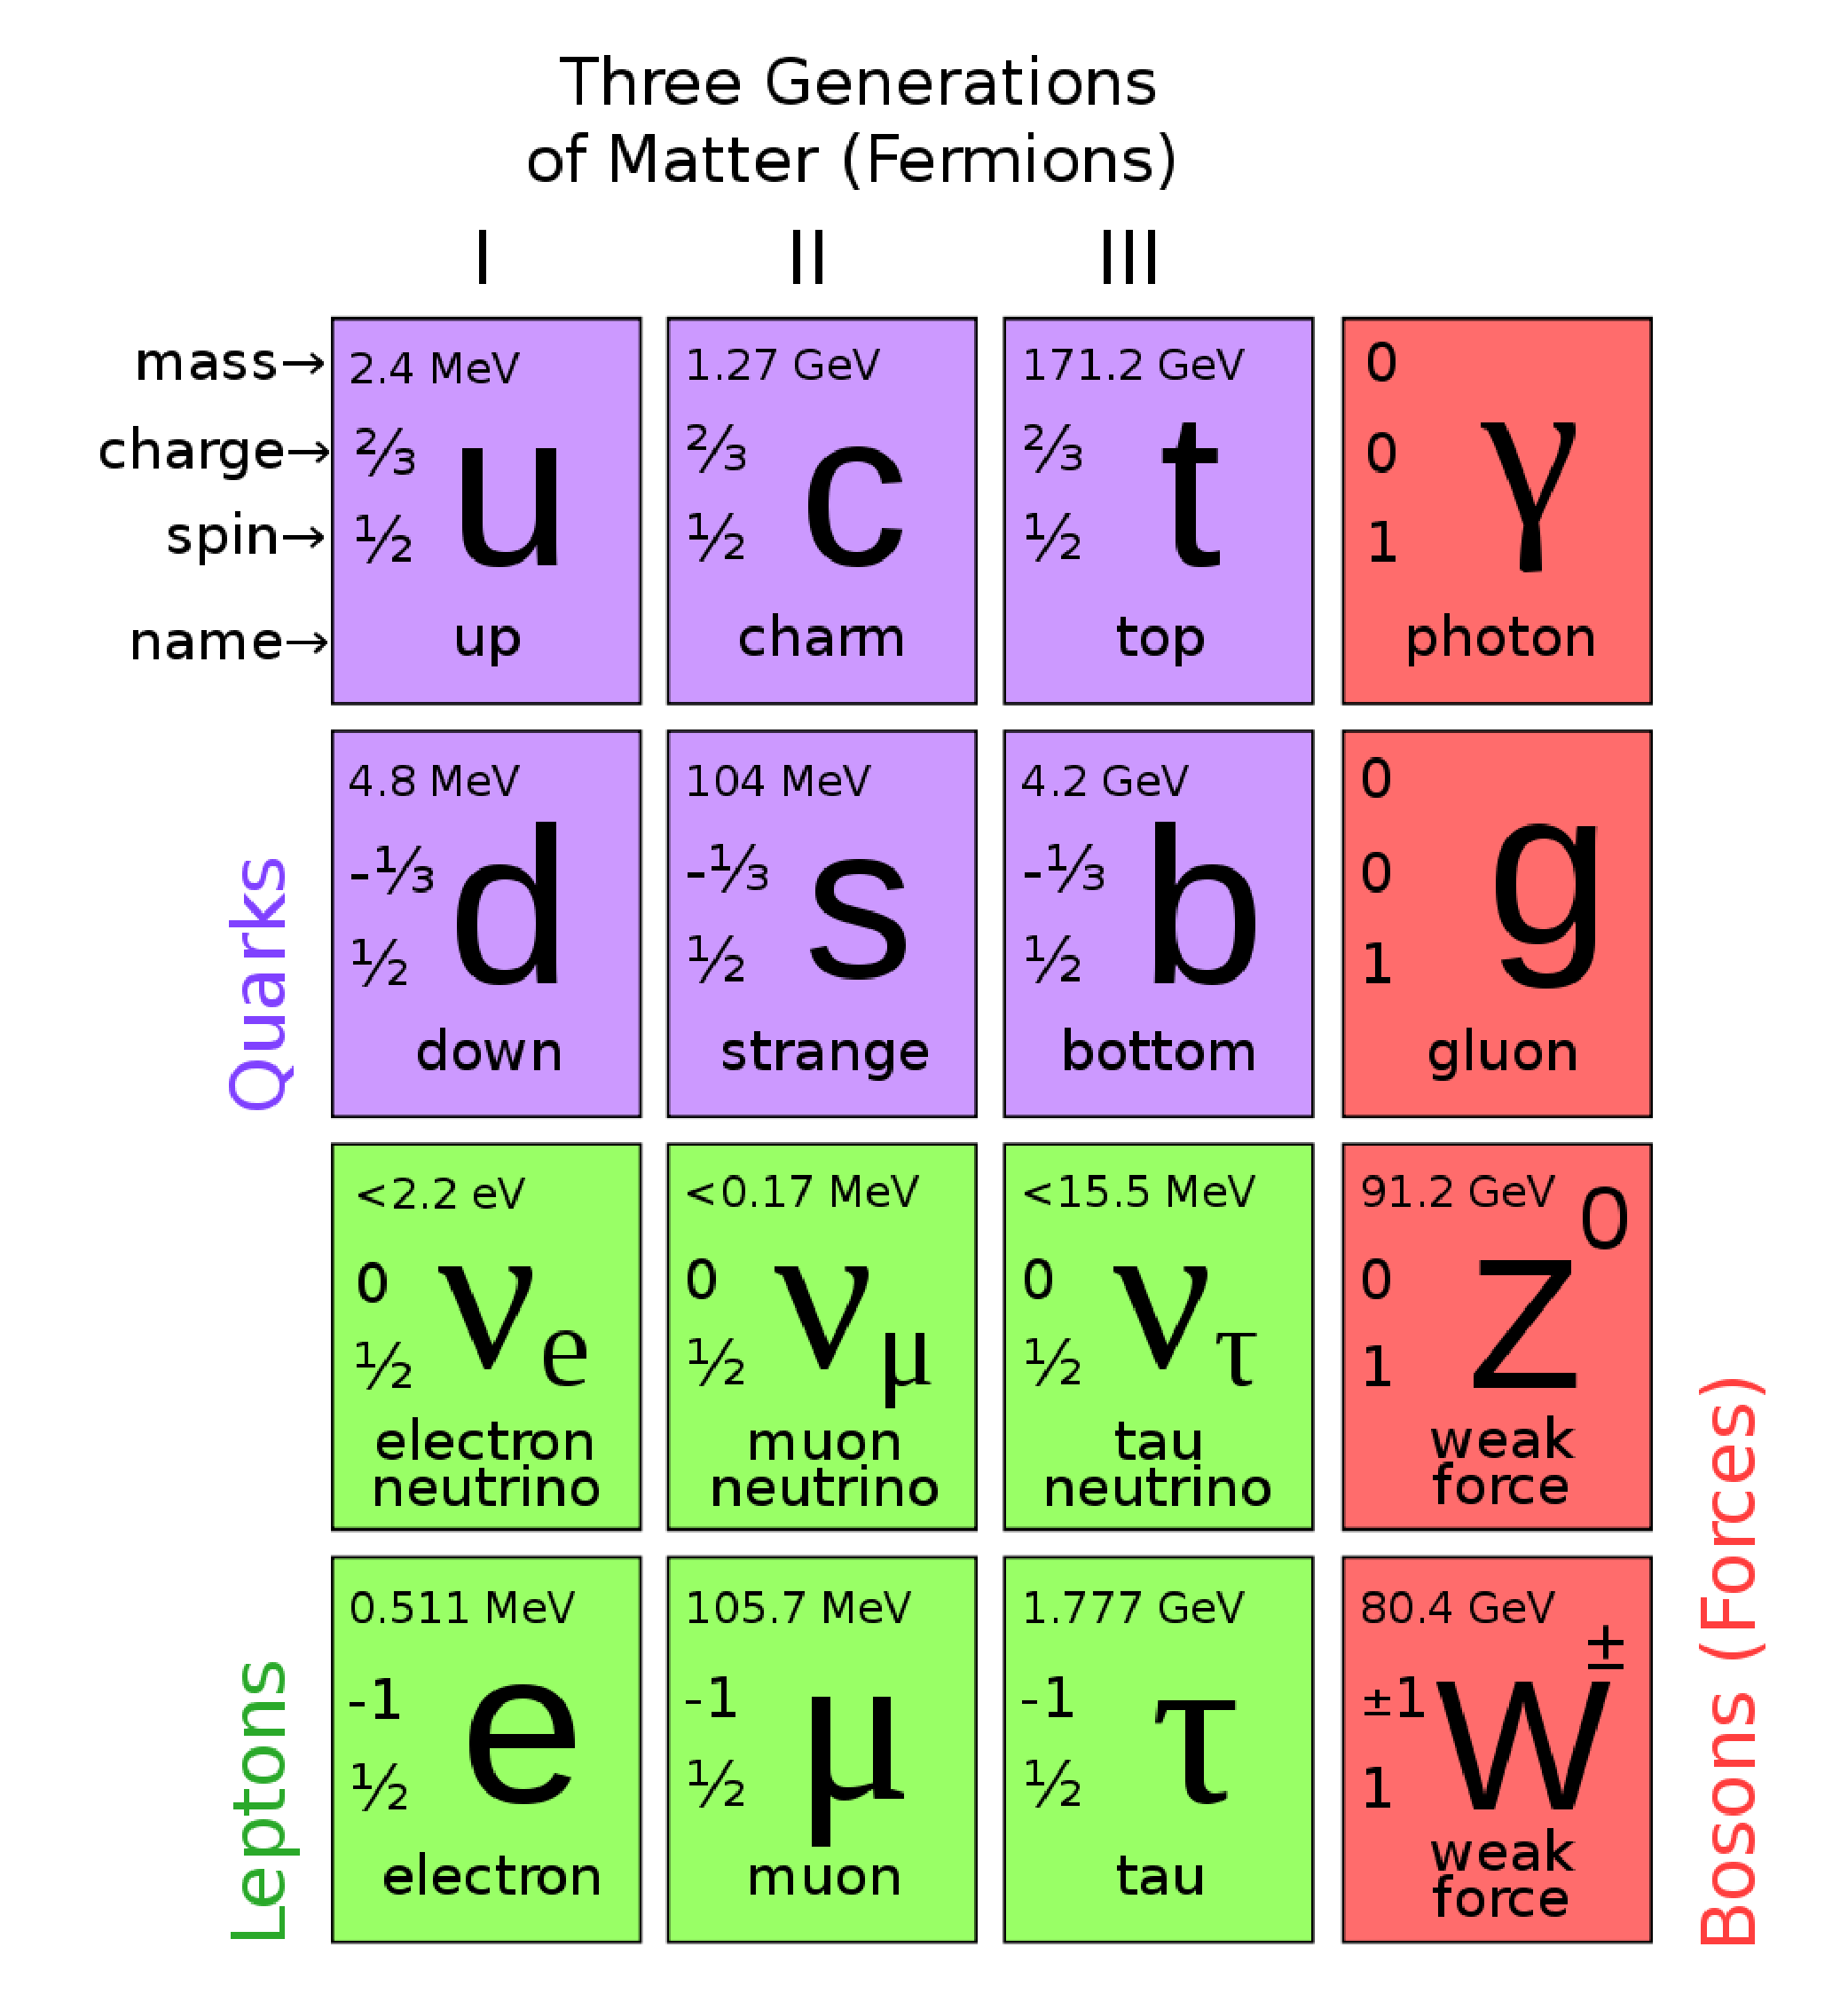
\includegraphics[width=.7\textwidth]{images/pdf/sm_particles}
    \caption{The particles in the unbroken SM.}
    \label{fig:sm_particles}
\end{figure}

\section{Spontaneous simmetry breaking: the Higgs mechanism}
We have only considered massless particles. This is not the case for all
the known fermions, and for the \W and \Z bosons. A mechanism was proposed
to preserve the gauge invariance of the lagrangian, while the vacuum state
is no longer a singlet under the action of the gauge group.

Spontaneous symmetry breaking of the local gauge symmetry in the SM provides massive
\W and \Z bosons and a new boson, called the Higgs boson.
In addition, we can obtain massive fermions by coupling them to the Higgs
field with Yukawa terms.

\section{The hierarchy problem}
Recently found evidence for a light Higgs boson, with a mass
near~\unit[125]{GeV}~\cite{higgs.atlas,higgs.cms}, are thought to be an indication of new symmetries and
new particles beyond the SM.

The theory predicts that the mass $m_H$ is subject to large radiative
corrections from loop diagrams similar to figure~\ref{fig:higgs_correction},
that should increase it by a large amount.
In the SM, fine tuning is required to prevent this corrections from becoming
too large~\cite{hierarchy}. Theoretical physicists generally dislike this fine tuning on grounds of
\emph{naturalness}.

\begin{figure}[htb]
    \centering
    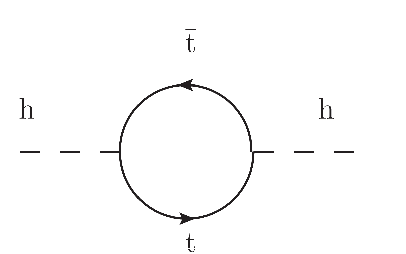
\includegraphics[width=.4\textwidth]{images/pdf/higgs_correction}
    \caption{Radiative correction to the Higgs mass from the top quark.}
    \label{fig:higgs_correction}
\end{figure}

The most notorious example of an extension to the SM that can eliminate this
naturalness problem is supersimmetry, where the radiative corrections to
the Higgs mass of the SM fermions are canceled by the contributions from
their superpartners.

There exist many theories that do not invoke supersimmetry as the solution
to the hierarchy problem. A robust and generic prediction of many of them is the
existence of new particles, the top partners, again balancing the
largest contribution to $m_H$ coming from the top quark.

\section{The top partners}\label{sec:top_partner_theory}
Theoretical developments predicting the existence of top partners stem from
the search for a way of introducing gravity in the SM, while solving the
hierarchy problem at the same time.

Five-dimensional space-time theories including gravity can be formulated in
terms of effective 4-d lagrangians where SM quarks mix with the top
partners, which, again from arguments of naturalness, should have a mass below or
slightly above the \unit[]{TeV} scale.
The lightest quarks have a small mass, indicating that their mixing with the
new particles is negligible. The top quark, having a very large mass, should have
a sizeable mixing with its partner, possibly making deviation
from the SM top interactions detectable at the LHC.

We use the top partner model from~\cite{Mrazek:2009yu} to describe our
signal, with vertices with the vector bosons and the top quark. 
We study the possibility of observing the top partners in the very clean
channel of two same-sign hard leptons. Typical production and decay diagrams
are shown in figure~\ref{fig:T53_production}.

\begin{figure}[htb]
    \centering
    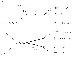
\includegraphics[width=.9\textwidth]{images/pdf/T53_production}
    \caption{Typical single and pair production of the top partner $\TP$ at the
    LHC.}
    \label{fig:T53_production}
\end{figure}
